\nonstopmode
\documentclass{article}

\usepackage[utf8]{inputenc}
\usepackage{geometry}
\usepackage{graphicx}
\usepackage{polski}
\usepackage{subcaption}

\graphicspath{ {images/} }
\geometry{legalpaper, portrait, margin=1in}

\title{\LARGE Złożone struktury danych \\ Sprawozdanie nr 2}
\author{Adam Piaseczny \\	151757 \and
				Igor Szczepaniak \\ 151918}
\date{Grupa piątkowa 11:45}

\begin{document}

\maketitle
\pagebreak

\tableofcontents
\pagebreak

\section{Wprowadzenie}

W tym sprawozdaniu zbadaliśmy sposoby wyszukiwania danych w różnych strukturach, byliśmy w stanie dzięki temu zweryfikować wiadomości poznane w trakcie zajęć. Kod źródłowy został napisany w języku \verb+python+ ze względu na prostotę implementacji.

Drogą prób i błędów doszliśmy do wniosku, że najbardziej optymalne dla naszych testów będzie ograniczenie maksymalnej ilości elementów do 20000 ze względu na problemy wiążące się z czasem wyszukiwania liniowego w tablicach o większej ilości elementów. Przewidzieliśmy 20 punktów pomiarowych, zaczynając od 1000 elementów z krokiem co 1000.

\section{Tworzenie struktur}

Dla wspomnianych wcześniej 20 wartości $n$ wygenerowaliśmy tablicę A zawierającą niepowtarzające się liczby całkowite dodatnie. Następnie wykonaliśmy kopię tej tablicy za pomocą \verb+numpy.ndarray.copy()+, którą potem posortowaliśmy korzystając z metody sortowania szybkiego (z elementem \verb+pivot+ na środku). Czas dodatkowego przypisania pamięci dla nowej tablicy $B$ oraz jej sortowania oznaczyliśmy jako $C_B$.

Korzytając z tablicy $A$ stworzyliśmy binarne drzewo poszukiwań, które w dalszej części pracy oznaczyliśmy jako $TA$. Zaimplementowaliśmy klasę \verb+Tree+, która posiada zmienną instancyjną \verb+root+ służącą do zapisywania korzenia drzewa binarnego będącego instancją \verb+Node+. Każdy obiekt \verb+Node+ zawiera od zera do dwóch potomków (\verb+self.left+, \verb+self.right+), przy czym każdy potomek "widzi" tylko swoich potomków (nie jest w stanie odnieść się do swojego rodzica). Każdy wierzchołek drzewa posiada również liczbę całkowitą (\verb+self.data+), według której jest porównywany z innymi wierzchołkami w strukturze. Wszystkie operacje na drzewie (wyszukiwanie, wprowadzanie danych oraz badananie wysokości struktury) rozpoczynają się na elemencie \verb+root+. Wprowadzanie wartości do drzewa, jak i jej wyszukiwanie, wartości opiera się na następującym algorytmie, gdzie rozpatrywany wierzchołek to \verb+self+:

\begin{enumerate}
	\item Jeśli wprowadzana wartość jest mniejsza od \verb+self.data+
		\begin{enumerate}
			\item Jeśli \verb+node.left+ nie istnieje, tworzymy nowy wierzchołek z wprowadzaną wartością jako \verb+self.data+, przypisujemy go jako \verb+node.left+ i kończymy wykonywanie funkcji.
			\item W przeciwnym wypadku wykonujemy ten sam algorytm dla już istniejącego \verb+node.left+.
		\end{enumerate}
	\item Jeśli wprowadzana wartość jest większa albo równa \verb+self.data+.
		\begin{enumerate}
			\item Jeśli \verb+node.right+ nie istnieje, tworzymy nowy wierzchołek z wprowadzaną wartością jako \verb+self.data+, przypisujemy go jako \verb+node.right+ i kończymy wykonywanie funkcji.
			\item W przeciwnym wypadku wykonujemy ten sam algorytm dla już istniejącego \verb+node.right+.
		\end{enumerate}
\end{enumerate}

Wyszukiwanie elementu w drzewie działa w sposób zbliżony do powyższego algorytmu, z tą różnicą, że jeżeli na drodze działania algorytmu natrafimy na \verb+Node+, który nie istnieje, kończymy algorytm z informacją, że szukanego elementu nie ma w strukturze. Jeśli natomiast natrafimy na \verb+self.data+ równa szukanej wartości kończymy algorytm zwracając \verb+self+.

Używając biblioteki \verb+sys+ dowiedzieliśmy się, że każdy element drzewa zajmuje 48 bajtów pamięci, podczas gdy każdy element tablicy zajmuje 8 bajtów pamięci. Łączna ilość pamięci zajęta przez drzewo to $(48\times n+1)$. Dodatkowe 48 bajtów pamięci jest zajmowane przez \verb+Tree+, które jest odnośnikiem do korzenia drzewa i służy do przeprowadzania operacji na drzewie poszukiwań. Dzięki temu odnośnikowi klasa \verb+Tree+ pozwala oszczędzić 16 bajtów na każdym wierzchołku w drzewie, które byłyby poświęcone odnośnikowi do \verb+Tree.root+.
Pomimo wyżej wspomnianego zaoszczędzenia pamięci struktura drzewa binarnego dla danego $n$ elementów będzie zawsze bardziej kosztowna pod względem pamięci niż tablica, gdyż łączny rozmiar tablicy to $8 \times n$.

Wprowadzając dane nieuporządkowane z tablicy $A$, idąc od pierwszego elementu do ostatniego w liście, zauważyliśmy, że wprowadzanie nowego elementu do drzewa $TA$ z czasem wymaga coraz więcej porównań oraz wywołań rekurencyjnych wyżej opisanego algorytmu (aż do $h$, gdzie $h$ jest wysokością drzewa, czyli najniższy poziom istniejący w drzewie). Przy tablicy $A$ nie możemy w kontrolowany sposób wpłynąć na maksymalną wysokość drzewa (ze względu na nieposortowany rozkład danych), przez co czas wprowadzania danych - $O(h)$, jest znacznie zwiększony.

Gdyby wprowadzać dane z tablicy $B$ w taki sam sposób jak z tablicy $A$ (od indeksu 0 do $n-1$) otrzymaliśmy drzewo o wysokości $n$, gdzie każdy wierzchołek miałby dokładnie jednego potomka \verb+node.right+. Jest to najgorszy możliwy przypadek wprowadzania danych do BST, ponieważ otrzymana struktura zajmuje więcej pamięci niż tablica. W takim drzewie można wyszukiwać dane tylko liniowo (sprawdzanie elementów jeden po drugim) oraz każda funkcja rekurencyjna (dodawanie elementów, wyszukiwanie albo sprawdzanie głębokości) wykonywałaby się aż $n$ razy. Mając to na względzie wprowadzając dane z tablicy $B$ użyliśmy dzielenia połówkowego tablicy posortowanej. Algorytm dzielenia połówkowego postępuje w następujący sposób:

\begin{enumerate}
	\item Wyznacza środkowy element tablicy
	\item Dodaje wybrany element do tablicy wynikowej
	\item Wykonuje dzielenie połówkowe dla elementów z lewej strony środkowego
	\item Wykonuje dzielenie połówkowe dla elementów z prawej strony środkowego
\end{enumerate}

Algorytm dzielenia połówkowego, tworząc tablice pomocniczą, gdzie każdy kolejny element stanowi medianę dzielonego fragmentu tablicy, sprawiło, że przypadek średni podczas budowania drzewa jest bliższy optymistycznemu niż pesymistycznemu znacząco zmniejszając wysokość drzewa. Wprowadzając kolejne elementy wyżej opisanej tablicy pomocniczej stworzyliśmy drzewo $TB$. Struktura ta przy wprowadzaniu kolejnych elementów podczas jego tworzenia wymagała mniejszej ilości porównań (niż w przypadku drzewa $TA$) zmniejszając tym samym wyskość drzewa $h$. Czas poświęcony na tworzenie drzewa $TB$ (pomijając czas tworzenia tablicy pomocniczej) oznaczony jest jako $C_{TB}$.

W następującej tabeli przedstawiliśmy zależność czasu $t$ od ilości elementów $n$ dla $C_B$, $C_{TA}$, $C_{TB}$.

\begin{figure}[h]
\centering
  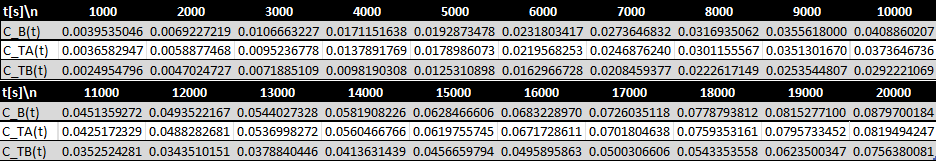
\includegraphics[width=1.0\linewidth]{tworzenie_tabela}
	\captionof{figure}{$t=f(n)$ - Tworzenie struktur (tabela)}
  \label{fig:tworzenie_tabela}
\end{figure}%

Z wyników z stworzyliśmy następujący wykres:

\begin{figure}[h]
\centering
  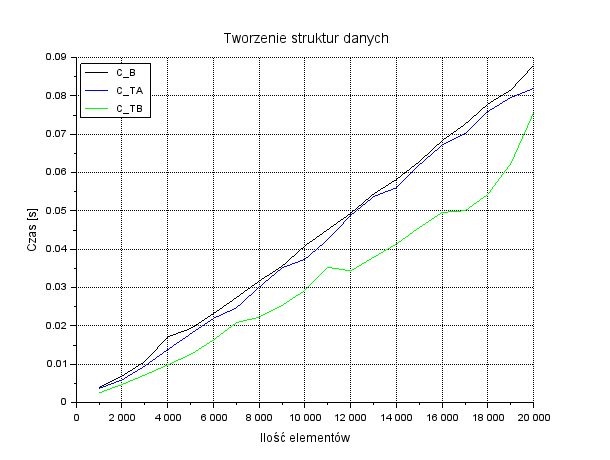
\includegraphics[width=0.5\linewidth]{tworzenie}
	\captionof{figure}{$t=f(n)$ - Tworzenie struktur}
  \label{fig:tworzenie}
\end{figure}%

Drzewo $TB$ podczas wprowadzania elementów musi wykonać w średnim przypadku mniej porównań między danymi w drzewie, niż drzewo $TA$. Z tego powodu czas tworzenia $TB$ jest niższy dla dowolnej ilości elementów $n$ w porównaniu do procesu tworzenia drzewa $TA$. W praktyce czas tworzenia drzewa $TB$ dla danych nieposortowanych wymaga stworzenia tablicy $B$ oraz uporządkowania jej, co wymaga dodatkowego czasu zawartego w $C_B$. Wymóg niezbędnego sortowania tablicy $B$ powoduje, że łączny czas tworzenia drzewa $TB$ jest większy od $TA$ dla danych nieposortowanych.

\section{Wyszukiwanie elementów}

W tym teście zmierzyliśmy jak długi czas zajmuje wyszukiwanie elementów w poszczególnych strukturach danych.

W tablicy $A$ zastosowalismy wyszukiwanie liniowe, czyli po pierwszym napotkanym szukanym elemencie zwracamy jego indeks i kończymy wykonywanie funkcji. Wyszukiwanie binarne dzieli tablicę posortowaną na dwie równe części według mediany i sprawdza czy szukana wartość jest większa czy mniejsza od mediany: jeśli jest większa to wywołujemy funkcje rekurencyjnie dla prawej strony tablicy, w przeciwnym przypadku wykonujemy dla lewej strony tablicy, przez rozpoczęciem wywołań rekurencyjnych sprawdzamy czy mediana jest równa szukanej wartosci, jeśli tak - zwracamy jej indeksi kończymy wykonywanie algorytmu. Szukanie każdego elementu z $A$ w $B$ za pomocą wyszukiwania binarnego oznaczone jest jako $S_B$ podczas gdy wyszukiwanie liniowe każdego elementu z $B$ w $A$ jest oznaczone jako $S_A$.

Dodatkowo wyszukujemy wszystkie elementy z $A$ w drzewie $TA$ ($S_{TA})$, oraz wszystkie elementy z $B$ w drzewie $TB$ ($S_{TB}$).

\begin{figure}[h]
\centering
  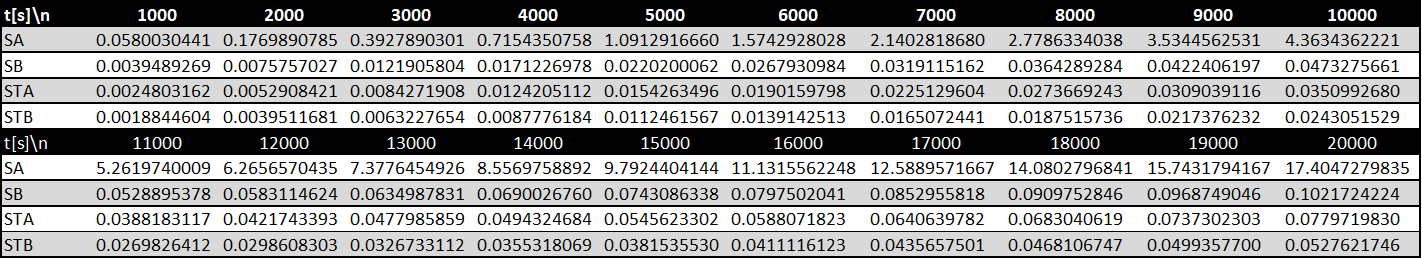
\includegraphics[width=1.0\linewidth]{wyszukiwanie_tabela}
	\captionof{figure}{$t=f(n)$ - Wyszukiwanie w strukturach (tabela)}
  \label{fig:szukanie_tabela}
\end{figure}%

\pagebreak
Z powyższych danych sporządziliśmy następujący wykres:

\begin{figure}[h]
\centering
  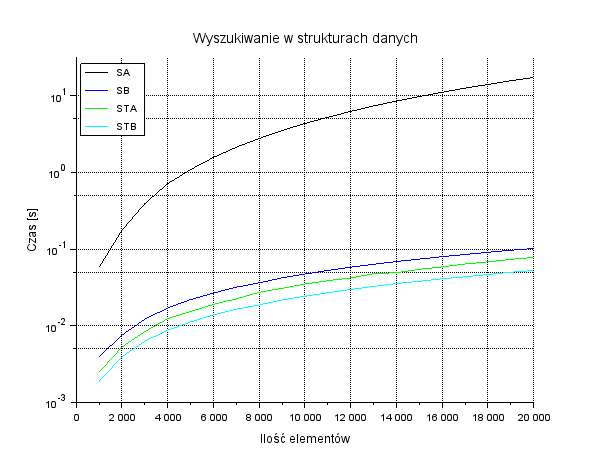
\includegraphics[width=0.5\linewidth]{wyszukiwanie}
	\captionof{figure}{$t=f(n)$ - Wyszukiwanie w strukturach}
  \label{fig:wyszukiwanie}
\end{figure}%

Wyszukiwanie liniowe w najgorszym przypadku ma złoność czasową $O(n)$. Takowy przypadek ma miejsce, kiedy wyszukiwany element znajduje się na końcu tablicy (aby go znaleźć należy sprawdzić aż $n$ elementów). Najgorszy przypadek dla wyszukwiania binarnego ma złożoność czasową $O(\log n)$. Dzieje się tak podczas najgłębszego zagnieżdżenia rekurencji, na przykład w przypadku szukania pierwszego albo ostatniego elementu tablicy.

Na wykresie możemy również zauważyć, że nawet przy losowym wprowadzaniu danych do drzewa $TA$ wyszukiwanie w nim jest szybsze niz wyszukiwanie binarne w liście $B$. Dzieje się tak z powodu faktu, że przy wykonywaniu rekurencyjnym wyszukiwania binarnego tworzą się kolejne funkcje na stosie rekurencyjnym co w przypadku języka \verb+python+ jest bardzo kosztowne dla pamięci. Dodatkowym "balastem pamięciowym" przypisanym do kolejnych wywołań jest również mediana, która oprócz zajmowania czasu na samo jej "obliczenie", rozszerza w kolejnym wywołaniu rekurencyjnemu słownik \verb+locals()+, zawierający zmienne w zasięgu lokalnym.

Jeśli wyszukujemy w binarnym drzewie poszukiwań $TA$, każde wywołanie rekurencyjne wyszukiwania \verb+Node.search()+ nie rozszerza słownika \verb+locals()+, z racji braku zmiennych lokalnych - wyszukiwanie w drzewie wykonuje tylko porównania. Przez nizszą średnią wysokość drzewa $TB$ spowodowaną dzieleniem połówkowym $B$ wyszukiwanie w drzewie $TB$ jest znacznie szybsze od wyszukiwania w drzewie $TA$ z racji mniejszej ilości porównań. Z tego powodu ten rodzaj wyszukiwania jest najszybszy ze wszystkich przez nas analizowanych.

\section{Wysokość}

W tym teście sprawdziliśmy w jaki sposób ilość elementów wpłynęła na wysokość drzew $TA$ oraz $TB$. Uśrednione wyniki naszych testów przedstawiliśmy w poniższej tabeli:

\begin{figure}[h]
\centering
  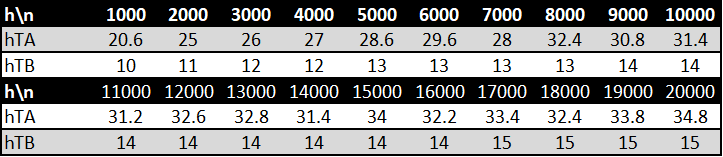
\includegraphics[width=0.9\linewidth]{wysokosc_tabela}
	\captionof{figure}{Wysokość struktur (tabela)}
  \label{fig:wysokosc_tabela}
\end{figure}%

Z powyższych danych sporządziliśmy następujący wykres:

\begin{figure}[h]
\centering
  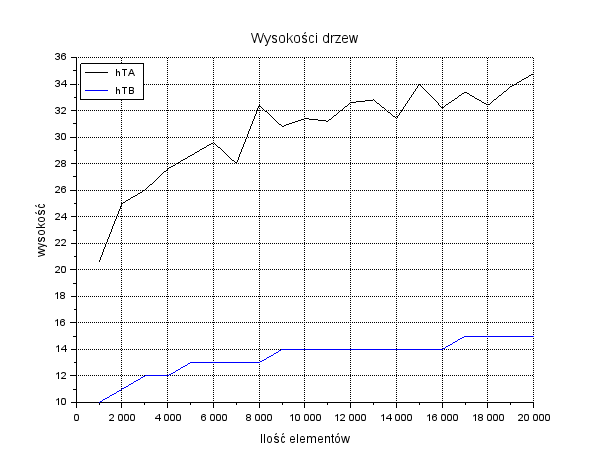
\includegraphics[width=0.5\linewidth]{wysokosc}
	\captionof{figure}{Wysokość struktur}
  \label{fig:wysokosc}
\end{figure}%
\pagebreak

Jak widać na powyższym wykresie wraz ze wzrostem ilości elementów wysokość drzewa $TA$ rośnie znacznie szybciej niż wysokość drzewa $TB$. Dzieje się tak, ponieważ rozkład danych w drzewie $TB$ jest bliżej przypadku optymistycznego przez użycie dzielenia połówkowego w jego tworzeniu. Wysokość drzew ma znaczący wpływ na szybkość operacji w tej strukturze danych co można dostrzec zestawiając powyższy wykres z danymi z wcześniejszych testów - duża wysokość drzewa powoduje dłuższy czas operacji na drzewie ze względu na ilość porównań.

Przy tworzeniu drzewa $TA$ nie były wymagane dodatkowe operacje przed rozpoczęciem iteracji przez tablicę $A$ aby dodać kolejne elementy do drzewa $TA$. Za to w przypadku drzewa $TB$ musiała zostać stworzona tablica pomocnicza jeszcze przed procesem dodawania elementów do drzewa. Jeśli chcielibyśmy dodać nowy element do stworzonego już drzewa $TB$ i utrzymać jego możliwie minimalną wysokość, musielibyśmy przejść przez proces dzielenia połówkowego posortowanej tablicy zawierającej nowy element w celu wyważenia drzewa, czyli optymializacji rozkładu danych w bst.

\section{Wnioski}

Używanie tablic jest prostsze w implementacji niż drzewo wyszukiwań, tablica zajmuje znacznie mniej pamięci niż drzewo binarne i pozwala na bezpośredni dostęp do danych (używając indeksu). Wyszukiwanie liniowe w nieposortowanej liście jest za to znacznie wolniejsze niż inne metody wyszukiwania rozważane w tej pracy, aczkolwiek jeśli dane są posortowane, rekurencyjne wyszukiwanie binarne jest porównywalnie szybkie do wyszukiwania w drzewach bst.

Drzewa bst są trudniejsze w implementacji oraz wymagają znacznie więcej pamięci na przechowywanie zmiennych instancyjnych. Dodatkowy czas poświęcony na tworzenie drzewa rekompensowany jest przez szybsze czasy wyszukiwania (nawet w drzewie $TA$ mimo dużej wysokości tej struktury). Najszybszą rozpatrywaną metodą jest wyszukwiwanie w drzewie doskonale zrównoważonym, którego wadą jest potrzeba ponownego wyważania drzewa jeśli będzie niezbędne dodanie elementów.

\section{Zakończnenie}

Wszystkie struktury mają swoje wady oraz zalety i warto rozważyć wiele czynników podczas decydowania, która struktura jest lepsza do danego zastosowania. Kod do wykorzystanego programu oraz pliki wyjściowe z danymi są dostępne pod witryną: \\\\
https://github.com/TypicalAM/Algorithms-Lab

\end{document}
